% ============================================================
%  DoRA Multi-Modal Research Poster — Cornell Red Theme
%  36 x 24 inches  (91.44 x 60.96 cm)
%
%  Cornell logo: drop cornell_seal.png in this folder.
%  If absent, the TikZ fallback seal is used automatically.
% ============================================================
\documentclass[final]{beamer}

\usepackage[size=custom,width=91.44,height=60.96,scale=1.2]{beamerposter}
\usepackage{amsmath,amssymb}
\usepackage{booktabs}
\usepackage{graphicx}
\usepackage{xcolor}
\usepackage{tikz}
\usepackage[most]{tcolorbox}
\usepackage{lmodern}
\usepackage{microtype}
\usepackage{ragged2e}
\usepackage{colortbl}
\usetikzlibrary{arrows.meta,positioning,shapes.geometric,calc}

% ----------------------------------------------------------
%  Cornell Palette
% ----------------------------------------------------------
\definecolor{CornellRed}  {RGB}{179, 27,  27}
\definecolor{CornellDark} {RGB}{ 91,  0,   0}
\definecolor{CornellMid}  {RGB}{140, 20,  20}
\definecolor{CornellAccent}{RGB}{220,170,170}
\definecolor{CornellGray} {RGB}{ 84, 88,  90}
\definecolor{BodyBg}      {RGB}{255,255,255}
\definecolor{TableShade}  {RGB}{253,238,238}

% ----------------------------------------------------------
%  Beamer base
% ----------------------------------------------------------
\setbeamercolor{background canvas}{bg=white}
\setbeamertemplate{navigation symbols}{}

% ----------------------------------------------------------
%  TikZ Cornell Seal (fallback)
% ----------------------------------------------------------
\newcommand{\CornellSealTikZ}[1][2.8cm]{%
  \begin{tikzpicture}
    \fill[CornellDark] (0,0) circle (#1);
    \fill[white]       (0,0) circle ({#1*0.84});
    \fill[CornellMid]  (0,0) circle ({#1*0.70});
    \fill[white]
      ({-#1*0.28},{#1*0.22}) -- ({-#1*0.28},{-#1*0.06})
      .. controls ({-#1*0.28},{-#1*0.32}) and (0,{-#1*0.44}) ..
      (0,{-#1*0.44})
      .. controls (0,{-#1*0.44}) and ({#1*0.28},{-#1*0.32}) ..
      ({#1*0.28},{-#1*0.06})
      -- ({#1*0.28},{#1*0.22}) -- cycle;
    \fill[CornellDark!80]
      ({-#1*0.28},{#1*0.22}) rectangle ({#1*0.28},{#1*0.10});
    \node[text=white,font=\fontsize{5}{5}\selectfont\bfseries]
      at (0,{#1*0.77}) {CORNELL UNIVERSITY};
    \node[text=white,font=\fontsize{4.5}{4.5}\selectfont]
      at (0,{-#1*0.77}) {FOUNDED A.D. 1865};
  \end{tikzpicture}%
}

\newcommand{\CornellLogo}[1][5.0cm]{%
  \IfFileExists{cornell.png}{%
    
\includegraphics[height=#1]{cornell.png}%
  }{%
    \CornellSealTikZ[#1]%
  }%
}

% ----------------------------------------------------------
%  Headline (9.5 cm — matches reference proportions)
% ----------------------------------------------------------
\setbeamertemplate{headline}{%
  \begin{beamercolorbox}[wd=\paperwidth]{headline}%
    \begin{tikzpicture}
      \fill[CornellRed]  (0,0) rectangle (\paperwidth, 9.5cm);
      \fill[CornellDark] (0,0) rectangle (\paperwidth, 0.28cm);
      % Cornell seal — vertically centred in the bar
      \node at (5.2cm, 5.2cm) {\CornellLogo[5.0cm]};
      % Title — large & bold, shifted right of seal
      \node[text=white,
            font=\fontsize{56}{62}\selectfont\bfseries,
            text width=76cm, align=left]
        at (14cm, 6.6cm)
        {Exploring DoRA: An Analysis of DoRA in Multi-Modal Domains};
      % Authors
      \node[text=white!90,
            font=\fontsize{28}{34}\selectfont, align=left]
        at (14cm, 3.4cm)
        {Richie Xue \quad\textbullet\quad
         Shaurya Sen \quad\textbullet\quad
         Kyle Du};
      % Affiliation (small)
      \node[text=white!65,
            font=\fontsize{16}{20}\selectfont, align=left]
        at (14cm, 1.6cm)
        {Cornell University \quad\textbullet\quad
         CS\,4782: Introduction to Deep Learning \quad\textbullet\quad
         Spring 2025};
    \end{tikzpicture}%
  \end{beamercolorbox}%
}

% ----------------------------------------------------------
%  Footline
% ----------------------------------------------------------
\setbeamertemplate{footline}{%
  \begin{beamercolorbox}[wd=\paperwidth,ht=1.8cm,dp=0.0cm]{footline}%
    \begin{tikzpicture}
      \fill[CornellDark] (0,0) rectangle (\paperwidth, 1.8cm);
      \node[text=white, font=\normalsize]
        at ({0.5*\paperwidth}, 0.9cm)
        {Cornell University $\cdot$ Dept.\ of Computer Science
         $\cdot$ CS\,4782: Introduction to Deep Learning
         $\cdot$ Spring 2025};
    \end{tikzpicture}%
  \end{beamercolorbox}%
}

% ----------------------------------------------------------
%  tcolorbox block style
% ----------------------------------------------------------
\tcbset{
  posterblock/.style={
    enhanced,
    colback        = BodyBg,
    colframe       = CornellDark,
    colbacktitle   = CornellMid,
    coltitle       = white,
    fonttitle      = \large\bfseries\itshape,
    boxrule        = 0.6pt,
    arc            = 5pt,
    titlerule      = 0pt,
    top            = 0.18cm,
    bottom         = 0.18cm,
    left           = 0.40cm,
    right          = 0.40cm,
    toptitle       = 0.14cm,
    bottomtitle    = 0.14cm,
    before skip    = 0.28cm,
  },
}

\newcommand{\hl}[1]{\textcolor{CornellRed}{\textbf{#1}}}
\newcommand{\lb}[1]{\textbf{#1:}\;}
\renewcommand{\arraystretch}{1.2}

% ----------------------------------------------------------
\begin{document}
\begin{frame}[t]
\vspace{0.2cm}

\begin{columns}[T,totalwidth=\textwidth]
\setlength{\columnsep}{0.8cm}

% ============================================================
%  COLUMN 1  —  Background + Methodology
% ============================================================
\begin{column}{0.31\textwidth}

\begin{tcolorbox}[posterblock,title=Background \& Motivation]
  \lb{Problem} Full fine-tuning of large pre-trained models
  (LLMs, ViTs, Wav2Vec) requires updating billions of parameters
  — prohibitive for most practitioners.

  \vspace{0.12cm}
  \lb{LoRA} Injects trainable low-rank matrices $\Delta W = BA$
  into frozen layers.  Efficient, but \emph{couples} the magnitude
  and direction of weight updates.

  \vspace{0.12cm}
  \lb{DoRA Key Insight} Decompose each weight into a learnable
  \hl{magnitude} scalar $m$ and a \hl{unit-norm direction}, then
  apply LoRA only to the direction:
  $\displaystyle W' = \underbrace{m}_{\text{scale}}
    \cdot \dfrac{W_0+BA}{\|W_0+BA\|_{\mathrm{col}}}$

  \vspace{0.04cm}
  $B$ initialised to $\mathbf{0}$; $m$ to column norms of $W_0$.
  Overhead vs.\ LoRA: $+d$ scalars per layer ($<0.1\%$).

  \vspace{0.12cm}
  \lb{Goals}
  \begin{itemize}
    \item Reproduce DoRA gains across four modalities
    \item Identify when magnitude decoupling matters
    \item Compare DoRA vs.\ LoRA at equal parameter budgets
  \end{itemize}
\end{tcolorbox}

\begin{tcolorbox}[posterblock,title=Methodology]
  \lb{Models \& Tasks}
  \begin{itemize}
    \item \textbf{NLP}: RoBERTa-base/large on GLUE (SST-2, MRPC, RTE)
    \item \textbf{Audio}: Wav2Vec2-base on Speech Commands (12 KWS)
    \item \textbf{Vision}: ViT-B/16 \& SigLIP-B/16 on robot grasping
    \item \textbf{VLA}: Action prediction on Push-T robot task
  \end{itemize}

  \vspace{0.12cm}
  \lb{Shared Config}
  Rank $r\!\in\!\{2,4,8,16,32\}$; $\alpha=2r$; target \texttt{q,k,v,o\_proj};
  AdamW + cosine LR; 5 epochs.

  \vspace{0.12cm}
  \lb{DoRA Decomposition Flow}

  \begin{center}
  \begin{tikzpicture}[
      box/.style={rectangle,rounded corners=2pt,draw=CornellDark,
                  fill=white,line width=0.6pt,minimum width=1.6cm,
                  minimum height=0.52cm,font=\small,align=center},
      arr/.style={-Stealth,thick,CornellGray}]
    \node[box,fill=CornellAccent!45](W0){$W_0$\\\scriptsize frozen};
    \node[box,right=0.7cm of W0](BA){$+BA$\\\scriptsize LoRA};
    \node[box,right=0.7cm of BA](N){$\div\|\cdot\|$\\\scriptsize norm};
    \node[box,fill=CornellRed!25,right=0.7cm of N](S){$\times m$\\\scriptsize scale};
    \draw[arr](W0)--(BA);
    \draw[arr](BA)--(N);
    \draw[arr](N)--(S);
  \end{tikzpicture}
  \end{center}

  \vspace{0.1cm}
  \lb{Implementation} Custom \texttt{DoRALinear} replaces every
  target \texttt{nn.Linear} in-place; magnitude $m$, $A$, $B$
  saved separately from frozen base weights.
\end{tcolorbox}

\end{column}

% ============================================================
%  COLUMN 2  —  NLP + Audio Results
% ============================================================
\begin{column}{0.37\textwidth}

\begin{tcolorbox}[posterblock,title=NLP Results — GLUE Benchmark]
  \lb{MRPC Rank Sweep} (RoBERTa-base; combined F1 + accuracy)

  \vspace{0.12cm}
  \begin{center}\small
  \begin{tabular}{@{}cccr@{}}
    \toprule
    \textbf{Rank} & \textbf{DoRA (\%)} & \textbf{LoRA (\%)} & $\Delta$ \\
    \midrule
    2  & 87.1 & 86.2 & $+0.9$ \\
    4  & 86.6 & 87.7 & $-1.1$ \\
    8  & 87.8 & 85.9 & $+1.9$ \\
    \rowcolor{TableShade}
    \textbf{16} & \textbf{90.3} & 87.3 & $\boldsymbol{+3.0}$ \\
    32 & 89.8 & 90.1 & $-0.3$ \\
    \bottomrule
  \end{tabular}
  \end{center}

  \vspace{0.08cm}
  \small\textit{DoRA at $r=16$ (90.3\%) beats LoRA's best ($r=32$: 90.1\%)
  at \textbf{half the parameters}.}

  \vspace{0.12cm}
  \lb{Cross-Task at $r=8$} (RoBERTa-base; best checkpoint)

  \vspace{0.08cm}
  \begin{center}\small
  \begin{tabular}{@{}lccc@{}}
    \toprule
    \textbf{Task} & \textbf{DoRA} & \textbf{LoRA} & $\Delta$ \\
    \midrule
    SST-2 (Acc) & 93.1\% & 93.3\% & $-0.2$ \\
    MRPC (F1) & \textbf{90.7\%} & 90.1\% & $+0.6$ \\
    \rowcolor{TableShade}
    RTE (Acc) & \textbf{71.1\%} & 70.8\% & $\boldsymbol{+0.3}$ \\
    \bottomrule
  \end{tabular}
  \end{center}

  \vspace{0.1cm}
  \small\textit{DoRA gains on \hl{low-data tasks}: +0.3\,pp RTE,
  +0.6\,pp MRPC F1. On large-data SST-2, LoRA converges equally
  well and magnitude decoupling provides no additional benefit.}

  \vspace{0.1cm}
  \lb{Real Validation Samples}
  {\footnotesize
  \begin{tabular}{@{}lp{5.3cm}l@{}}
    \textbf{SST-2} & ``\textit{...crowd-pleasing as a documentary can get.}'' & $\to$ \hl{Positive} \\[1pt]
    \textbf{MRPC}  & S1: ``\textit{Corixa rose 54c to \$7.74.}'' S2: ``\textit{...rose 54c, or 8\%, to \$7.74.}'' & $\to$ \hl{Not Equiv.} \\[1pt]
    \textbf{RTE}   & P: ``\textit{Leaders signed Egypt--Israel treaty in 1979.}'' H: ``\textit{Treaty signed in 1979.}'' & $\to$ \hl{Not Entailed} \\
  \end{tabular}}
\end{tcolorbox}

\begin{tcolorbox}[posterblock,title=Audio Results — Speech Commands]
  Wav2Vec2-base (67M params) fine-tuned on Google Speech Commands
  v0.02 — 84.8k utterances, \textbf{12 keyword classes}.

  \vspace{0.12cm}
  \begin{center}\small
  \begin{tabular}{@{}lcccc@{}}
    \toprule
    \textbf{Method} & \textbf{Val Acc} & \textbf{Test Acc}
                    & \textbf{Trainable} & \textbf{Time} \\
    \midrule
    \rowcolor{TableShade}
    DoRA ($r=8$) & \textbf{98.6\%} & \textbf{89.7\%}
                 & 826.6k & \textbf{152.8 min} \\
    LoRA ($r=8$) & 98.5\% & 89.0\%
                 & 789.8k & 190.8 min \\
    \bottomrule
  \end{tabular}
  \end{center}

  \vspace{0.08cm}
  \small\textit{\hl{+0.7\% test accuracy}, \hl{25\% less training time}.
  Faster directional gradient convergence on the audio encoder.}
\end{tcolorbox}

\end{column}

% ============================================================
%  COLUMN 3  —  Vision/VLA Samples + Conclusions
% ============================================================
\begin{column}{0.29\textwidth}

\begin{tcolorbox}[posterblock,title=Vision \& Robot Results]
  \lb{Cornell Grasp} Success rate (IoU$\!\geq\!0.25$ \& $|\Delta\theta|\!\leq\!30°$):

  \vspace{0.08cm}
  \begin{center}\small
  \begin{tabular}{@{}lccc@{}}
    \toprule
    \textbf{Backbone} & \textbf{DoRA} & \textbf{LoRA} & \textbf{Full FT} \\
    \midrule
    ViT-B/16    & 7.9\%  & 6.2\%  & 0.6\% \\
    \rowcolor{TableShade}
    SigLIP-B/16 & 19.8\% & \textbf{20.3\%} & 15.8\% \\
    \bottomrule
  \end{tabular}
  \end{center}

  \vspace{0.06cm}
  \small\textit{SigLIP ($3\times$ over ViT) dominates; DoRA $\approx$ LoRA.
  Full FT collapses on 885 images.}

  \vspace{0.10cm}
  \lb{Qualitative: SigLIP + DoRA}
  {\small\textit{Green} = predicted\quad\textit{Red} = ground truth}

  \vspace{0.1cm}
  \begin{center}
  \begin{tabular}{@{}cccc@{}}
    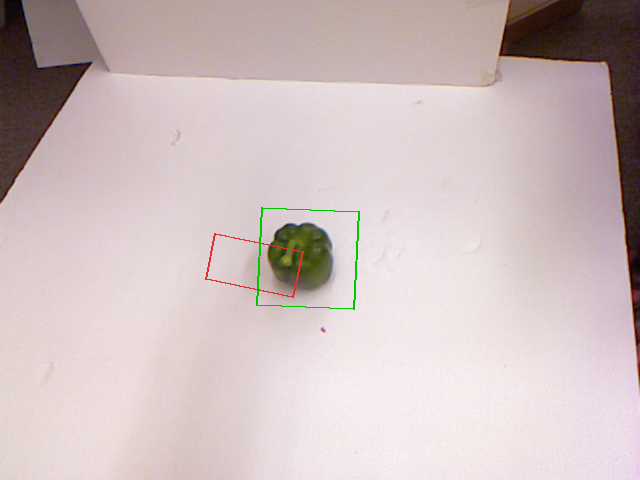
\includegraphics[width=1.85cm,height=1.45cm,
      clip]{grasp_siglip_00.png} &
    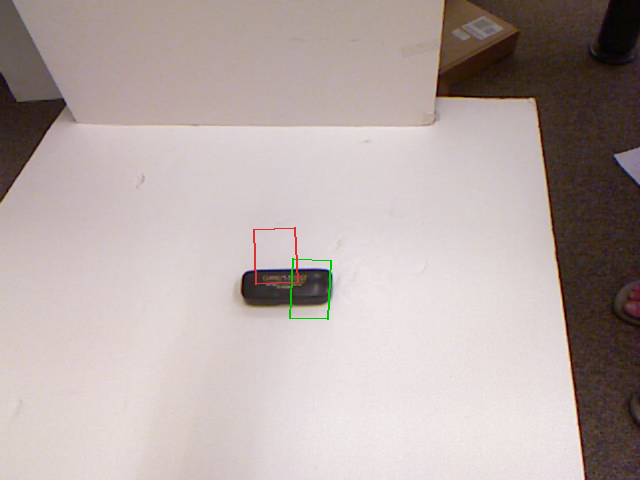
\includegraphics[width=1.85cm,height=1.45cm,
      clip]{grasp_siglip_04.png} &
    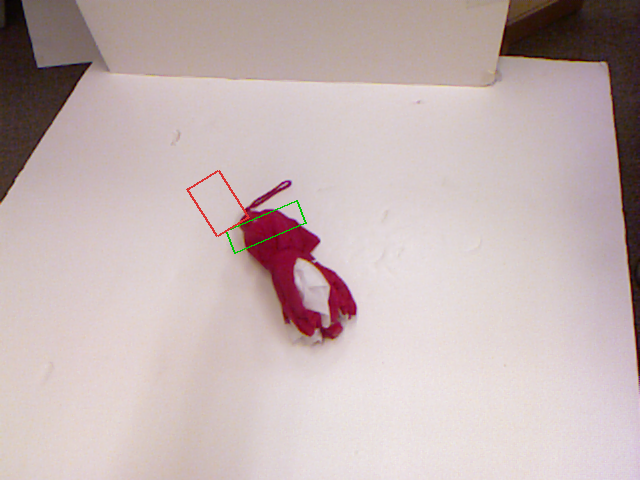
\includegraphics[width=1.85cm,height=1.45cm,
      clip]{grasp_siglip_07.png} &
    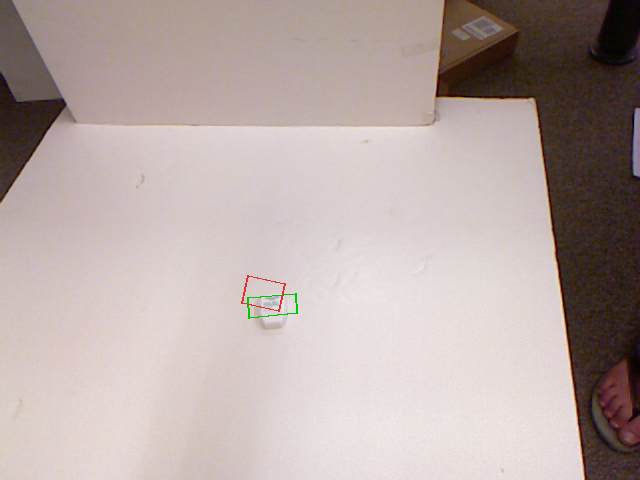
\includegraphics[width=1.85cm,height=1.45cm,
      clip]{grasp_siglip_09.png}
  \end{tabular}
  \end{center}

  \vspace{0.15cm}
  \lb{Push-T VLA Task}
  DoRA and LoRA applied to a 126-layer VLA for robotic push-block
  manipulation.  Action MSE after 3 epochs:
  DoRA $63.6\!\to\!27.9$; \hl{LoRA $62.1\!\to\!\mathbf{24.8}$}
  (LoRA outperforms — too few epochs for magnitude decoupling to
  take effect).

  \vspace{0.1cm}
  \begin{center}
  \begin{tabular}{@{}ccc@{}}
    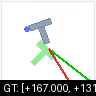
\includegraphics[width=2.2cm,height=1.75cm,
      clip]{pusht_03.png} &
    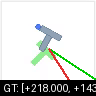
\includegraphics[width=2.2cm,height=1.75cm,
      clip]{pusht_04.png} &
    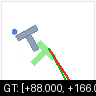
\includegraphics[width=2.2cm,height=1.75cm,
      clip]{pusht_07.png}
  \end{tabular}
  \end{center}
  \vspace{0.08cm}
  \centering{\small\textit{DoRA adapter driving Push-T rollouts}}
\end{tcolorbox}

\begin{tcolorbox}[posterblock,title=Conclusions \& References]
  \begin{itemize}\setlength\itemsep{1pt}
    \item \hl{Low-data NLP}: +0.3\,pp RTE, +0.6\,pp MRPC F1
          (both $r=8$); DoRA at $r=16$ matches LoRA at $r=32$
          with half the parameters
    \item \hl{Audio}: $+0.7\%$ test accuracy, $25\%$ faster
          training on Wav2Vec2 + Speech Commands
    \item \hl{Vision}: SigLIP benefits more than ViT; gains are
          modality- and architecture-dependent
    \item Gains \hl{diminish on large models} where LoRA saturates
    \item DoRA is a \hl{drop-in LoRA replacement} across all four
          modalities tested
  \end{itemize}

  \vspace{0.12cm}
  {\small
  [1] Liu et al.\ (2024). DoRA: Weight-Decomposed Low-Rank Adaptation.
      \textit{ICML 2024}.\\[2pt]
  [2] Hu et al.\ (2022). LoRA.  \textit{ICLR 2022}.\\[2pt]
  [3] Wang et al.\ (2018). GLUE Benchmark. \textit{EMNLP}.\\[2pt]
  [4] Warden (2018). Speech Commands. \textit{arXiv}.}
\end{tcolorbox}

\end{column}

\end{columns}

\end{frame}
\end{document}
